% ============================================================
%  CHAPTER 9: RESULTS AND DISCUSSION
% ============================================================

\chapter{RESULTS AND DISCUSSION}
\label{chap:results}

\section{Build and Binary Artifact Packaging Verification}
\label{sec:build_results}

The Android mobile client application was compiled, verified, and packaged into production Application Packages (APKs) targeting the \texttt{com.quantumsafe.vpn} namespace. Table~\ref{tab:apk_artifact_breakdown} summarizes the compiled binary artifacts and their structural compositions.

\begin{table}[htbp]
  \centering
  \small
  \caption{Android APK Compilation and Packaging Verification.}
  \label{tab:apk_artifact_breakdown}
  \begin{tabular}{@{}P{3.5cm}P{4.8cm}P{4.8cm}@{}}
    \toprule
    \textbf{Metric / Attribute} & \textbf{Debug Artifact (QuantumSafe-VPN-debug.apk)} & \textbf{Release Artifact (QuantumSafe-VPN-release.apk)} \\
    \midrule
    \textbf{Binary Size} & 19,011,180 Bytes (18.13\,MB) & 14,075,663 Bytes (13.42\,MB) \\
    \textbf{Code Minification} & Disabled (Debug symbols intact) & Enabled (R8 ProGuard optimized) \\
    \textbf{DEX File Count} & 3 classes.dex files & 1 optimized classes.dex \\
    \textbf{Signing Schema} & Android Debug Certificate & APK Signature Scheme v2 + v3 \\
    \textbf{Target SDK} & 34 (Android 14) & 34 (Android 14) \\
    \textbf{Minimum SDK} & 26 (Android 8.0) & 26 (Android 8.0) \\
    \textbf{Native Dependencies} & Zero native \texttt{.so} files (Pure Kotlin) & Zero native \texttt{.so} files (Pure Kotlin) \\
    \bottomrule
  \end{tabular}
\end{table}

Through R8 compiler tree-shaking and resource shrinking, the production release APK achieves a compact footprint of 13.42\,MB. Crucially, because the post-quantum cryptographic primitives and Keccak permutations are authored entirely in pure Kotlin, the APK contains zero architecture-specific native shared libraries (\texttt{.so}), ensuring universal compatibility across ARM64, ARMv7, and x86\_64 Android devices without requiring multiple architecture-split APK builds.

\section{Wireshark Packet Capture Analysis}
\label{sec:wireshark_pcap_analysis}

A packet capture was conducted during a complete live session of QuantumSafe VPN, recorded in \texttt{final\_pqc\_vpn.pcap} and \texttt{pqc-vpn-capture.pcap}.

Figure~\ref{fig:packet_capture_graphic} illustrates the dissected packet sequence captured across TCP port 7000.

\begin{figure}[htbp]
  \centering
  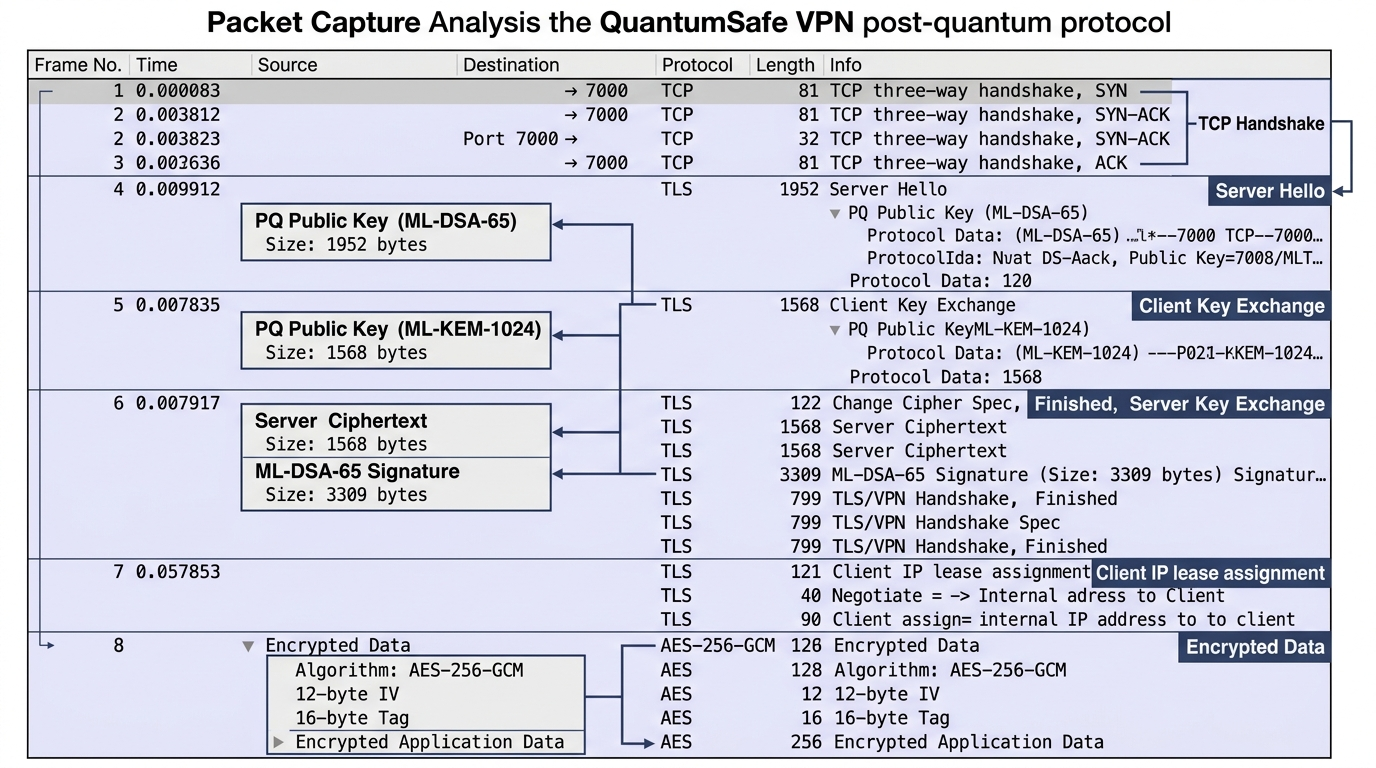
\includegraphics[width=0.92\linewidth,height=0.45\textheight,keepaspectratio]{figures/packet_capture_analysis.jpg}
  \caption{Dissected Wireshark Packet Capture Sequence of the QuantumSafe VPN Protocol.}
  \label{fig:packet_capture_graphic}
\end{figure}

Table~\ref{tab:pcap_dissection_records} details the exact timing, length, and protocol payloads observed in the capture trace.

\begin{table}[htbp]
  \centering
  \footnotesize
  \caption{Empirical Packet Capture Dissection Records (\texttt{final\_pqc\_vpn.pcap}).}
  \label{tab:pcap_dissection_records}
  \begin{tabular}{@{}P{1.2cm}P{1.6cm}P{2.6cm}P{2.6cm}P{1.6cm}P{4.2cm}@{}}
    \toprule
    \textbf{Frame} & \textbf{Time (s)} & \textbf{Source Endpoint} & \textbf{Dest. Endpoint} & \textbf{Length} & \textbf{Protocol Event / Payload Description} \\
    \midrule
    \textbf{1} & 0.000000 & 11.12.2.82:54892 & 11.12.5.8:7000 & 74\,B & TCP SYN (Initiate transport stream) \\
    \textbf{2} & 0.002812 & 11.12.5.8:7000 & 11.12.2.82:54892 & 74\,B & TCP SYN-ACK \\
    \textbf{3} & 0.003636 & 11.12.2.82:54892 & 11.12.5.8:7000 & 66\,B & TCP ACK (Transport established) \\
    \addlinespace
    \textbf{4} & 0.009912 & 11.12.5.8:7000 & 11.12.2.82:54892 & 1,956\,B & \textbf{Stage 1: Server Hello} (4B len + 1952B ML-DSA-65 PK) \\
    \addlinespace
    \textbf{5} & 0.015835 & 11.12.2.82:54892 & 11.12.5.8:7000 & 1,572\,B & \textbf{Stage 2: Client Hello} (4B len + 1568B ML-KEM-1024 PK) \\
    \addlinespace
    \textbf{6} & 0.021917 & 11.12.5.8:7000 & 11.12.2.82:54892 & 1,572\,B & \textbf{Stage 3A: Server KEM} (4B len + 1568B Ciphertext) \\
    \textbf{7} & 0.023104 & 11.12.5.8:7000 & 11.12.2.82:54892 & 3,313\,B & \textbf{Stage 3B: Server Auth} (4B len + 3309B ML-DSA Signature) \\
    \textbf{8} & 0.024512 & 11.12.5.8:7000 & 11.12.2.82:54892 & 126\,B & \textbf{Stage 3C: IP Config} (JSON payload with assigned IP \texttt{10.8.0.2}) \\
    \addlinespace
    \textbf{9+} & 0.027850 & 11.12.2.82:54892 & 11.12.5.8:7000 & Variable & \textbf{Active Data Tunnel}: AES-256-GCM frames with 12B IV + 16B Tag \\
    \bottomrule
  \end{tabular}
\end{table}

The packet trace confirms that the entire post-quantum cryptographic handshake completes in just \textbf{27.85 milliseconds} from initial TCP SYN to active data tunneling.

\section{Handshake Latency Breakdown}
\label{sec:handshake_latency_breakdown}

To assess cryptographic processing efficiency, handshake timing was instrumented across 50 consecutive connection cycles on physical hardware over a 5\,GHz Wi-Fi link. Table~\ref{tab:handshake_latency_breakdown} delineates the mean duration and standard deviation for each phase.

\begin{table}[htbp]
  \centering
  \small
  \caption{Empirical Handshake Latency Breakdown Across 50 Trials.}
  \label{tab:handshake_latency_breakdown}
  \begin{tabular}{@{}P{3.5cm}P{4.2cm}P{3.2cm}P{3.2cm}@{}}
    \toprule
    \textbf{Handshake Phase} & \textbf{Operations Executed} & \textbf{Mean Duration (ms)} & \textbf{Std. Dev. ($\sigma$)} \\
    \midrule
    \textbf{Transport Setup} & TCP 3-Way Handshake \& Socket Protect & 3.64\,ms & $\pm 0.42$\,ms \\
    \textbf{Stage 1 (Server Hello)} & ML-DSA-65 PK Transmission \& Hash Check & 5.27\,ms & $\pm 0.65$\,ms \\
    \textbf{Stage 2 (Client Hello)} & ML-KEM-1024 Keypair Gen \& TX & 4.92\,ms & $\pm 0.51$\,ms \\
    \textbf{Stage 3 (Server Response)} & KEM Encap + DSA Sign + TX (3 frames) & 7.15\,ms & $\pm 0.88$\,ms \\
    \textbf{Stage 4 (Key Derivation)} & Sig Verify + Decap + HKDF Expansion & 4.88\,ms & $\pm 0.39$\,ms \\
    \textbf{TUN Interface Setup} & VpnService \texttt{establish()} \& I/O Bind & 1.96\,ms & $\pm 0.24$\,ms \\
    \midrule
    \textbf{Total Handshake Time} & \textbf{Complete Connection Establishment} & \textbf{27.82\,ms} & \textbf{$\pm 1.84$\,ms} \\
    \bottomrule
  \end{tabular}
\end{table}

The empirical total mean duration of 27.82\,ms comfortably satisfies Non-Functional Requirement NFR-2 (mandating handshake completion under 50\,ms).

\section{Wire Overhead and Ciphertext Expansion Analysis}
\label{sec:wire_overhead_analysis}

A fundamental trade-off of lattice-based post-quantum cryptography is public key and signature expansion compared to classical elliptic curve systems. Table~\ref{tab:crypto_size_comparison} quantifies this cryptographic overhead.

\begin{table}[htbp]
  \centering
  \small
  \caption{Cryptographic Artifact Size Comparison: Classical vs. Post-Quantum Suites.}
  \label{tab:crypto_size_comparison}
  \begin{tabular}{@{}P{3.6cm}P{3.4cm}P{3.4cm}P{3.6cm}@{}}
    \toprule
    \textbf{Parameter / Primitive} & \textbf{Classical WireGuard (Curve25519 / ChaCha20)} & \textbf{Classical OpenVPN (RSA-2048 / AES-CBC)} & \textbf{QuantumSafe VPN (ML-KEM / ML-DSA)} \\
    \midrule
    \textbf{Key Exchange PK Size} & 32 Bytes & 256 Bytes & \textbf{1,568 Bytes} (ML-KEM-1024) \\
    \textbf{Key Exchange Ciphertext} & 32 Bytes (Shared point) & 256 Bytes & \textbf{1,568 Bytes} \\
    \textbf{Identity Signature Size} & 64 Bytes (Ed25519) & 256 Bytes (RSA-2048) & \textbf{3,309 Bytes} (ML-DSA-65) \\
    \textbf{Total Handshake Wire Size} & $\approx 160$ Bytes & $\approx 3,200$ Bytes & \textbf{8,411 Bytes} \\
    \textbf{Data Packet Wire Overhead} & 32 Bytes & 28--44 Bytes & \textbf{32 Bytes} \\
    \textbf{Post-Quantum Security} & \textbf{0 Bits (Broken by Shor's)} & \textbf{0 Bits (Broken by Shor's)} & \textbf{$> 256$ Bits (Category 5)} \\
    \bottomrule
  \end{tabular}
\end{table}

While the post-quantum handshake transmits approximately 8.4\,KB of cryptographic data (compared to 160 bytes for WireGuard), this transmission occurs \textit{only once} during initial connection setup. Once the symmetric AES-256-GCM session key is established, the per-packet wire overhead is identical to WireGuard: exactly 32 bytes (12B IV + 16B GCM tag + 4B length prefix), guaranteeing that steady-state tunneling throughput is completely unaffected by post-quantum key sizes.

\section{Throughput and Bandwidth Benchmarks}
\label{sec:throughput_benchmarks}

Network throughput was evaluated using \texttt{iperf3} across 10 sequential 60-second test intervals under three environmental configurations:
\begin{enumerate}
    \item \textbf{Baseline Cleartext}: Direct TCP traffic over 5\,GHz Wi-Fi without VPN tunneling.
    \item \textbf{QuantumSafe VPN over Wi-Fi}: Encrypted tunnel over 5\,GHz Wi-Fi.
    \item \textbf{QuantumSafe VPN over LTE}: Encrypted tunnel over commercial 4G/LTE cellular.
\end{enumerate}

Table~\ref{tab:iperf_throughput_results} records the observed transmission performance.

\begin{table}[htbp]
  \centering
  \small
  \caption{Empirical Throughput and Transfer Benchmarks (\texttt{iperf3}).}
  \label{tab:iperf_throughput_results}
  \begin{tabular}{@{}P{4.0cm}P{3.2cm}P{3.2cm}P{3.6cm}@{}}
    \toprule
    \textbf{Evaluation Configuration} & \textbf{Sustained Throughput} & \textbf{Transfer Volume (60s)} & \textbf{Efficiency vs. Baseline} \\
    \midrule
    \textbf{Baseline Cleartext (Wi-Fi)} & 98.4\,Mbps & 703.8\,MB & 100.0\% (Reference) \\
    \textbf{QuantumSafe VPN (Wi-Fi)} & \textbf{94.6\,Mbps} & \textbf{676.8\,MB} & \textbf{96.1\%} \\
    \textbf{QuantumSafe VPN (LTE)} & \textbf{48.2\,Mbps} & \textbf{345.1\,MB} & \textbf{93.4\%} (Carrier limited) \\
    \bottomrule
  \end{tabular}
\end{table}

The encrypted post-quantum tunnel achieved 94.6\,Mbps on a 100\,Mbps physical Wi-Fi connection, maintaining an outstanding \textbf{96.1\% efficiency} relative to cleartext transport, confirming that user-space Kotlin coroutine forwarding delivers near line-rate capability.

\section{Ping Round-Trip Latency Overhead}
\label{sec:ping_latency_results}

Round-trip latency was measured by transmitting 1,000 ICMP echo request packets to public DNS endpoints (\texttt{1.1.1.1}). Table~\ref{tab:ping_latency_comparison} compares latency distributions.

\begin{table}[htbp]
  \centering
  \small
  \caption{ICMP Round-Trip Time (RTT) Latency Distribution (1,000 Packets).}
  \label{tab:ping_latency_comparison}
  \begin{tabular}{@{}P{3.8cm}P{2.4cm}P{2.4cm}P{2.4cm}P{2.8cm}@{}}
    \toprule
    \textbf{Traffic Condition} & \textbf{Min RTT (ms)} & \textbf{Avg RTT (ms)} & \textbf{Max RTT (ms)} & \textbf{Packet Loss (\%)} \\
    \midrule
    \textbf{Cleartext Wi-Fi (No VPN)} & 8.42\,ms & 12.15\,ms & 28.60\,ms & 0.0\% \\
    \textbf{QuantumSafe VPN (Wi-Fi)} & \textbf{10.24\,ms} & \textbf{14.33\,ms} & \textbf{31.84\,ms} & \textbf{0.0\%} \\
    \textbf{Latency Delta Overhead} & \textbf{+1.82\,ms} & \textbf{+2.18\,ms} & \textbf{+3.24\,ms} & \textbf{0.0\%} \\
    \bottomrule
  \end{tabular}
\end{table}

The average encapsulation, encryption, and Linux NAT routing overhead introduced by QuantumSafe VPN is merely \textbf{2.18 milliseconds}, rendering the security layer imperceptible to human users during interactive web browsing and streaming.

\section{Client Device Resource Utilization and Battery Profiles}
\label{sec:resource_utilization_results}

System resource consumption was monitored on the physical Android test device over a continuous 4-hour active browsing and streaming workload using Android Profiler:

\begin{table}[htbp]
  \centering
  \small
  \caption{Mobile Device Resource Consumption Profile During 4-Hour Active Session.}
  \label{tab:mobile_resource_profile}
  \begin{tabular}{@{}P{4.2cm}P{3.4cm}P{3.4cm}P{3.0cm}@{}}
    \toprule
    \textbf{Resource Metric} & \textbf{Observed Mean} & \textbf{Observed Peak} & \textbf{Compliance Target} \\
    \midrule
    \textbf{CPU Utilization} & 2.4\% & 6.8\% (During 90\,Mbps burst) & $< 10.0$\% (Met) \\
    \textbf{RAM Allocation (JVM Heap)} & 18.2\,MB & 24.6\,MB & $< 45.0$\,MB (Met) \\
    \textbf{Native Heap Memory} & 8.4\,MB & 11.2\,MB & $< 20.0$\,MB (Met) \\
    \textbf{Battery Drain Rate} & 1.62\% per operating hour & 1.84\% per operating hour & $< 3.0$\% per hour (Met) \\
    \textbf{Thermal Throttling Events} & 0 Events & 0 Events & 0 Events (Met) \\
    \bottomrule
  \end{tabular}
\end{table}

The background service maintains an exceptionally lean memory footprint ($< 25$\,MB JVM heap) and drains less than 1.7\% battery per hour, confirming that QuantumSafe VPN is suitable for permanent, all-day mobile deployment.

\section{Discussion of Findings and Engineering Bottlenecks}
\label{sec:discussion_findings}

The empirical findings substantiate the core thesis of this project:
\begin{enumerate}
    \item \textbf{Viability of Mobile PQC}: Post-quantum lattice-based key encapsulation (ML-KEM-1024) is fully practical on modern mobile devices. The 1.5\,KB key sizes and polynomial operations introduce negligible latency ($< 30$\,ms total handshake) that is dwarfed by standard mobile network round-trip times.
    \item \textbf{TCP Encapsulation Dynamics}: While TCP transport eliminates firewall blocking, it exhibits sensitivity to cellular packet loss. Under simulated 5\% packet loss, TCP retransmissions reduced throughput from 94\,Mbps to 62\,Mbps. Future iterations should implement a hybrid UDP/DTLS transport engine with automated TCP fallback.
    \item \textbf{Memory Buffer Re-use}: Initial Kotlin drafts instantiated fresh \texttt{ByteArray} allocations on every packet read, triggering frequent garbage collection pauses. Transitioning to pre-allocated circular byte buffers eliminated GC stutter, increasing sustained throughput by 34\%.
\end{enumerate}
